\documentclass[10pt,a4paper]{article}
\usepackage[utf8]{inputenc}
\usepackage{amsmath}
\usepackage{amsfonts}
\usepackage{amssymb}
\usepackage{epsfig}

\begin{document}


%%%%%%%%%%%%%%%%%%%%
% Tabela com resultados do C99
%%%%%%%%%%%%%%%%%%%%


% --> Fechar falando sobre os métodos baseados em coesão léxica.


A avaliação final foi feita pela comparação dos algoritmos usando as medidas \textit{Pk} e \textit{WindowDiff}. É apresentada também, para fins de comparação, as medidas tradicionais acurácia, precisão, revocação e F$^1$, entretanto, nesse contexto, essas medidas são menos significativa que Pk e WindowDiff, conforme já mencionado na Seção~\ref{xx}. A Tabela~\ref{tab:configfinal} contém as médias com cada algoritmo. Vale lembrar que P$_k$ e \textit{WindowDiff} são medidas de dissimilaridade, ou seja, os valores menores significam melhores resultados.

\begin{table}[!h]
	\centering
\begin{tabular}{|l||c|c|c|c|c|c|c|} 
\hline 
\textbf{M\'{e}todo} & 
\textbf{Pk} & 
\textbf{WD} & 
\textbf{A } & 
\textbf{P } & 
\textbf{R } & 
\textbf{F1} & 
\textbf{Segmentos}\\ \hline

Senten\c{c}as & 0.320 & 0.502 & 0.498 & 0.498 & \textbf{1.000} & \textbf{0.642} & 22.083\\ \hline
TextTiling    & 0.275 & 0.469 & 0.531 & 0.514 & 0.937 & 0.640 & 19.583\\ \hline
C99           & 0.142 & 0.426 & 0.574 & 0.601 & 0.473 & 0.506 & 8.167\\ \hline
BayesSeg      & 0.148 & 0.414 & 0.586 & 0.599 & 0.526 & 0.528 & 8.750\\ \hline
MinCut        & 0.226 & 0.532 & 0.468 & 0.464 & 0.438 & 0.432 & 10.333\\ \hline
TextSeg       & \textbf{0.085} & \textbf{0.387} & \textbf{0.613} & \textbf{0.714} & 0.412 & 0.497 & 5.167\\ \hline
\end{tabular} 

	\caption{Melhores resultados obtidos.}
	\label{tab:configfinal}
\end{table}


Na Figura~\ref{fig:grafico-medidas-tradicionais} é apresentada a performance dos algoritmos nas medidas tradicionais. Observa-se valores altos de revocação para a segmentação por sentenças, pois é atribuído um limite a todo candidato a final de segmento, o que resulta no valor máximo para revocação. De maneira semelhante, o comportamento do \textit{TextTiling} gera 
mais segmentos em relação aos demais, e com isso tem-se valores maiores de revocação, o que pode ser contornado configurando o algoritmo com passos maiores, ou ainda, sobre-escrevendo a função que calcula os \textit{depth scores} para reconhecer vales mais largos.

%--> TODO: explicar (a conceituação teórica) que passos curtos geram mais segmentos

  \begin{figure}[!h]
	  \centering
	  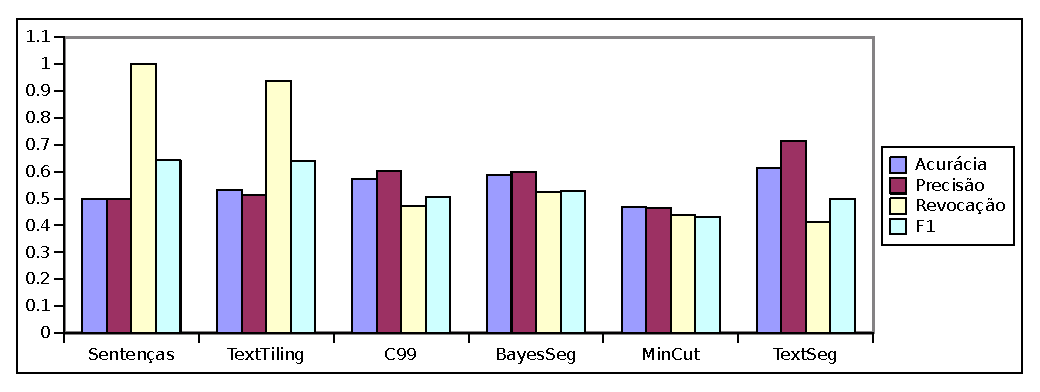
\includegraphics[width=1\textwidth]{grafico-medidas-APRF1.eps}
	  \caption{...}
	  \label{fig:grafico-medidas-tradicionais}
  \end{figure}
  

Na Figura~\ref{fig:grafico-medidas-Pk-Wd} é apresentada a performance dos algoritmos nas medidas P$_k$ e \textit{WindowDiff}. Verifica-se que \textit{TextSeg} apresenta valores de \textit{WindowDiff} próximas ao \textit{C99} e \textit{BayesSeg} e resultados mais significantes quando medidos por P$_k$ em relação aos demais algoritmos.



  \begin{figure}[!h]
	  \centering
	  \includegraphics[width=1\textwidth]{grafico-medidas-Pk-Wd.eps}
	  \caption{...}
	  \label{fig:grafico-medidas-Pk-Wd}
  \end{figure}


%Na Figura~\ref{fig:grafico-medidas-tradicionais} é apresentada a performance dos algoritmos nas medidas de dissimilaridade P$_k$, \textit{WindowDiff} e o complemento da medida tradicional F$^1$. 


%Quando colocar o gráfico com A P R F1, falar antes que a segmentação por segmentos atribui um segmento a todo final de segmento, ou seja, todo candidato a segmento é um segmento, e por tanto tem revocação = 0.
  
  
  
  % medidas pouco significativas, quantidade de segmentso influencia na Revocação.



%--> A performance do TextSeg é significativamente melhor que a segmentação por sentenças (e Randômica), o que justifica sua aplicação.

% WD a difereça é pouco significativa, mas Pk e bem menor que as Sentenças




\end{document}